% Template for ICASSP-2018 paper; to be used with:
%          spconf.sty  - ICASSP/ICIP LaTeX style file, and
%          IEEEbib.bst - IEEE bibliography style file.
% --------------------------------------------------------------------------
\documentclass{article}
\usepackage{spconf,amsmath,graphicx}

% Example definitions.
% --------------------
\def\x{{\mathbf x}}
\def\L{{\cal L}}

% Title.
% ------
\title{SINGLE SOURCE AUDIO SEPARATION}
%
% Single address.
% ---------------
\name{Author(s) Name(s)\thanks{Thanks to XYZ agency for funding.}}
\address{Author Affiliation(s)}
%
% For example:
% ------------
%\address{School\\
%	Department\\
%	Address}
%
% Two addresses (uncomment and modify for two-address case).
% ----------------------------------------------------------
%\twoauthors
%  {A. Author-one, B. Author-two\sthanks{Thanks to XYZ agency for funding.}}
%	{School A-B\\
%	Department A-B\\
%	Address A-B}
%  {C. Author-three, D. Author-four\sthanks{The fourth author performed the work
%	while at ...}}
%	{School C-D\\
%	Department C-D\\
%	Address C-D}
%
\begin{document}
%\ninept
%
\maketitle
%
\begin{abstract}
We propose an audio separation methodology from a single source audio signal (SSAS) based on a generative adversarial network (GAN).  For the generator structure we have proposed a deep attractor network (DANet), which performs the signals separation process. This generator has the advantages to work on a non fixed number of sources during the training or testing stages, without special constrains on  vocabulary and grammar. For the discriminator  structure we have used two bidirectional long short term memory (BLSTM) networks for processing text and signal respectively. 
The proposed methodology showed a very efficient end-to-end training scheme and highly reduced  computation complexity compared with other methods.

\end{abstract}
%
\begin{keywords}
Single source audio separation, generative adversarial network, deep attractor network, bidirectional long short term memory network.
\end{keywords}
%
\section{Introduction}
The problem of a single source audio separation (SSAS) arises in many problems (Insert Examples and references here). Diverse deep neural networks (DNNs) based techniques have shown  to achieve good performances solving this problem, however many of them are constrained to the target number of sources,  inefficiency to perform end-to-end mapping and computation efficiency. There exist two main approaches for using DNNs  for SSAS (Insert References here). The first approach trains the DNNs to map the features of the mixed signal into the features of the sources directly whereas the second maps the mixed signal into spectral masks that explain the contribution of each source in the mixed signal. 
Since the training stage uses the reference sources directly for the first approach then the DNN becomes less sensitive to the variation of the mixed ratio in the mixed signals. For the second approach DNNs are trained to produce bounded values (masks between zero and one) rather than training to predict the sources which can take any real values.

In this paper we propose a methodology for SSAS based on a generative adversarial network (GAN). 
A generative adversarial network (GAN) is a method for estimation of a generative model by adversarial process (Insert Reference here). It is composed of two networks: a generator and a discriminator. The generator network $G$ maps a noise variable $z$ $\mathtt{\sim}$ $P(z)$ to data space $x=G(z)$ whereas the discriminator $D$ assigns a probability $p=D(x) \in [0,1]$ when $x$ is a real training sample and assigns $1-p$ when $x$  comes from the generator $G$.  $P(z)$ is typically a uniform distribution [1,-1]. 
The overall objective is to ensure that $D$ finds a binary classifier which provides the best  discrimination between real and generated data at the time that $G$ is fitted to the true data distribution. 
In our proposal the generator is the signals separator component and the speech recognizer while the discriminator is composed of two subnetworks, a discriminator subnetwork for the speech signal and another one for the text. The output of both are then fused using a fully-connected layer.

We propose a deep attractor network (DANet) based structure for the generator $G$ for the signals separation process. The main advantages of this approach are that it does not assume anything about the number of sources during training or testing stages and does not imposes special constraints on vocabulary and grammar. For the discriminator $D$ we use two bidirectional long short term memory  (BLSTM) networks in order to process the text and the signal obtaining two embedding vectors. Then we feed concatenated embedding vector to a fully connected layer, which output a 3 dimensional categorical probability distribution belonging to classes {true\_signal, true\_noise, fake\_signal}.

The paper is organized as follows. In Section II provides an overview of the methods


%In this paper we propose to use a Wasserstein GAN, that uses a different loss/cost functions that perform well in training better than regular GANs (Insert Reference here or are the results of the proposal?). 



 

\label{sec:intro}

%% Refined the results

\section{Related work}
\label{sec:related}
\subsection{LSTM Denoising Autoencoder feature-mapping network (DAE)}
Previous works have used the long-short term memory (LSTM) denoising autoencoders, which has  shown better performance than the feature-mapping networks (Insert Reference here). This separator requires the assumption that the number of sources are fixed. Autoencoders (AE) based on  recurrent neural networks (RNN)  can deal with sequences while regular AE can not. In this approach the 
RNN share their parameters/weights across all timesteps because what they are trying to learn is time-invariant. A speech signal can show-up in any moment of time. On a RNN the weights are learned with back propagation through time (BPTT). The BPTT gradients get too small (or too large) as the propagation  occurs from $t$ to $t-T$ where $T$ is large. This network tends to forget previous “events” due to shrinkage of earlier hidden node activations as time progresses. To preserve the earlier ($t-T$) hidden node activations and to be able to use them in predictions at time $t$ it is needed to use Long short-term memory RNNs. 
The LSTM RNNs are designed for remembering long-time dependencies and can be leveraged to incrementally update the learnt models for both noise and speech sources over time and learn the context. Therefore it uses uses potentially longer context (Longer than?).  

This method uses a mask-learning network which  is bounded (e.g. the mask usually has value in [0; 1]). Therefore, it is easier for the mask learning network to generalize different noises and conditions  on a fixed dynamic range. Moreover, during the separation since the mixture is re-introduced to the computation, the network only needs to filter out the noisy part. Compared with the feature mapping network, where the system needs to both remove the noise and remember the clean reference, the learning task for mask based system is easier, and thus usually leads to better performance.

The main disadvantages of this method are that it fails to handle the permutation problem which occurs when separating more than two sources. This method also requires the number of sources that is used in the training to be the same number of sources in testing. On the feature-mapping network side,  the network directly output the clean spectrogram, which is unbounded, the output dynamic range has to be large enough to cover all possible volumes. Such procedure will largely increase the redundancy for the learning task. For example, for the same utterance with different amplitude, the feature mapping network need to generate completely different result, which will make the network more difficult to converge. Also, prediction of the spectra may also yield over-smoothing effects in general due to the regression-to-the-mean effect (regardless of predicting log-spectra or not).

\subsection{Deep clustering-based separator (DC)}
DC can solve both permutation and the output dimension problem to produce the state of the art separation performance. 
However, the main drawback of DC is its inefficiency to perform end-to-end mapping, because the objective function is the affinity between the sources in the embedded space and not the separated signals themselves. Minimizing the separation error is done with an unfolding clustering system and a second network, which is trained iteratively and stage by stage to ensure convergence.

\subsection{Permutation Invariant Training (PIT)}
This algorithm algorithm solves the permutation problem by pooling over all possible permutations for $N$ mixing sources ($N!$ permutations), and use the permutation with lowest error to update the network. It has been shown to have comparable performance as DC.  However, this approach suffers the output dimension mismatch problem because it assumes a fixed number of sources. Another disadvantage of this method is the computation efficiency, where  the prediction window has to be much shorter than context window due to the inconsistency of the permutation both across and within sample segments

\subsection{Deep Attractor based separator (DANet)}
The DANet solves the permutation problem and does not suffer from the output dimensions mismatch problem. It can potentially be extended to arbitrary number of sources without the permutation problem. The mask learning enables a very efficient end-to-end training scheme and highly reduces the computation complexity compared with DC and PIT. DANet removes the stepwise pre-training required in DC method to enable end-to-end training. Another big advantage of DANet arises from the flexibility in source dependent training, where the source-dependent knowledge could be easily incorporated by the attractor (e.g. speaker identity). 
This separator does not assume anything about the number of sources during training or test times. This approach does not imposes special constraint on vocabulary and grammar. The separator performs a speaker-independent separation.

\subsubsection{Estimation of the attractor points}
During the training stage, the attractor points can be estimated using various methods including the average. One possibility is to use weighted average. Since the attractors represents the source center of gravity, we can include only the embeddings of the most salient $T-F$ bins, which leads to more robust estimation. We investigate this strategy by using an amplitude threshold in the estimation of the attractor. 
Alternatively, a neural network model may also be used to pick the representative embedding for each source, an idea which shares similarities with encoder-decoder attention networks.

For the testing stage, because the true assignment $Y$ is unknown, we incorporate two strategies to form the attractor points. The first find the centers using post $K$-means algorithm. The second method is based on the observation that the location of the attractors in the embedding space is relatively stable.


\section{Model design}

\subsection{Generator}
\subsubsection{DANet Architecture}
\begin{itemize}
\item The network consists of 4  BLSTM layers with 600 hidden units in each layer.
\item The embedding dimension is set to 20, resulting in a fully-connected feed-forward layer of 2580 hidden units (20 x 129) after the BLSTM layers.
\end{itemize}

\subsection{Discriminator}
We use two BLSTM subnetworks in order to process the signal and the text obtaining two embedding vectors and a final fully connected  layer which output a 3 dimensional categorical probability distribution belonging to classes {true\_signal, true\_noise, fake\_signal}.
\subsubsection{BLSTM  Signal Architecture}
\begin{itemize}
\item The network contains 4  BLSTM layers with 600 hidden units in each layer.
\item The embedding dimension is set to 20, resulting in a fully-connected feed-forward layer of 2580 hidden units (20 x 129) after the BLSTM layers.
\end{itemize}

\subsubsection{BLSTM  Text Architecture}
\begin{itemize}
\item  2 BLSTM layers will have 600 and 300 hidden units respectively.
\end{itemize}
\label{sec:format}

\subsubsection{Classification layer}


\begin{figure}[htb]
\begin{minipage}[b]{1.0\linewidth}
  \centering
  \centerline{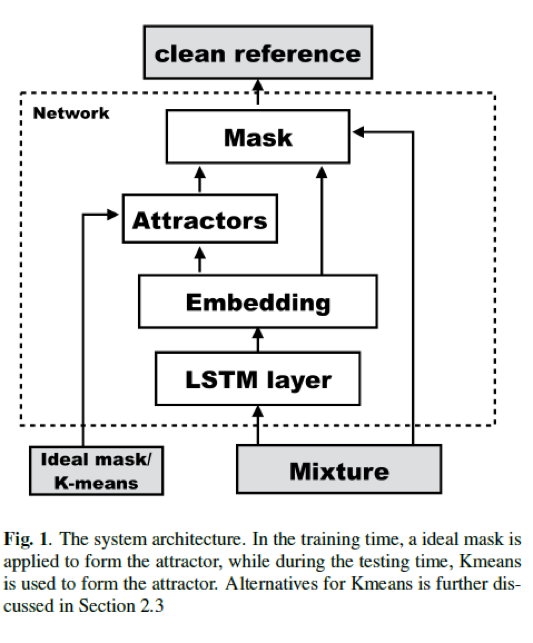
\includegraphics[width=8.5cm]{Picture1.png}}
%  \vspace{2.0cm}
  \centerline{(a) Result 1}\medskip
\end{minipage}
%
\caption{System architecture.}
\label{fig:res}
%
\end{figure}


\section{Data Collection }
\label{sec:pagestyle}
\subsubsection{DANet Dataset}
It contains a 30 h training set and a 10 h validation set generated by randomly selecting utterances from
different speakers in the Wall Street Journal (WSJ0) training  set si\_tr\_s, 
and mixing them at various signal-to-noise ratios (SNR) randomly chosen between 0 dB and 10 dB. 5 h evaluation set is generated similarly as above, using utterances from 16 unseen speakers from si\_dt\_05 and si\_et\_05 in WSJ0 dataset. Additionally, the authors constructed a three-speaker mixture dataset for three speaker separation evaluation from same WSJ set, which has 30h training, 10 hours validation and 5 hours testing data, with mixing SNR at -5 5 dB. They ensure that in each mixture, there exist both female and male speakers. All data are resampled to 8 kHz to reduce computational and memory costs.

\section{Experimentation}
\label{sec:typestyle}




\subsection{DANet Standalone Training}
RMSprop algorithm is used for training with an exponential learning rate decaying strategy, where the learning rate starts at $10^{-4}$ and ends at 3 x $10^{-6}$. The total number of epochs was set to be 150, and we will use the cost function in Eq. \ref{Eq:CostFunction} on the validation set for early stopping. 
\begin{equation}
\mathcal{L}=\sum_{f,t,c} || S_{f,t,c}-X_{f,t} \times M_{f,t,c}||^2_2 \label{Eq:CostFunction}
\end{equation}
where $S$ is the clean spectrogram (frequency $F\times$ time $T$) of $C$ sources, $X$ is the mixture spectrogram (frequency $F\times$ time $T$), and $M$ is the mask formed to extract each source.
The criteria for early stopping is no decrease in the loss function on validation set for 10 epochs.  Moreover, by applying curriculum training strategy, i.e. continue training the network with 400-frame length input, DANet achieves the best overall performance.

\subsection{Metrics}
The signal-to-distortion ratio (SDR, which is defined as scale-invariant SNR here), signal-to-artifacts ratio (SAR), and signal-to-interference ratio (SIR).

\section{Evaluation}
\label{sec:majhead}



\section{Conclusion}
\label{sec:print}



\vfill\pagebreak

\section{References}
\label{sec:refs}



% References should be produced using the bibtex program from suitable
% BiBTeX files (here: strings, refs, manuals). The IEEEbib.bst bibliography
% style file from IEEE produces unsorted bibliography list.
% -------------------------------------------------------------------------
\bibliographystyle{IEEEbib}
\bibliography{strings,refs}

\end{document}
